\documentclass[aspectratio=169]{beamer}

% Theme and Color
\usetheme{Madrid}
\usecolortheme{beaver}

% Packages
\usepackage{graphicx}
\usepackage{booktabs}
\usepackage{tikz}
\usepackage{pgfplots}
\pgfplotsset{compat=1.17}
\usetikzlibrary{shapes.geometric, arrows, positioning, fit, calc}

% Title Data
\title[MoodTune AI]{MoodTune AI: Emotion-Aware Music Recommendation System}
\subtitle{Personalized Audio Experience using Reinforcement Learning}
\author{MoodTune Project Team}
\institute{Department of Computer Science}
\date{\today}

\begin{document}

% Slide 1: Title
\begin{frame}
    \titlepage
\end{frame}

% Slide 2: Introduction & Problem Statement
\section{Introduction}
\begin{frame}{Problem Statement \& Solution}
    \begin{columns}
        \column{0.5\textwidth}
        \textbf{The Problem}
        \begin{itemize}
            \item Standard shuffles play random tracks regardless of context.
            \item Static playlists fail to adapt to real-time mood shifts.
            \item Manual song selection breaks focus and immersion.
        \end{itemize}

        \column{0.5\textwidth}
        \textbf{Our Solution: MoodTune AI}
        \begin{itemize}
            \item \textbf{Dynamic}: Adapts to user's emotional state in real-time.
            \item \textbf{Intelligent}: Learns preferences via Reinforcement Learning.
            \item \textbf{Personalized}: Builds a unique model for every user.
        \end{itemize}
    \end{columns}
\end{frame}

% Slide 3: System Architecture (Detailed)
\section{System Architecture}
\begin{frame}{System Architecture}
    \begin{center}
    \resizebox{0.75\textwidth}{!}{
    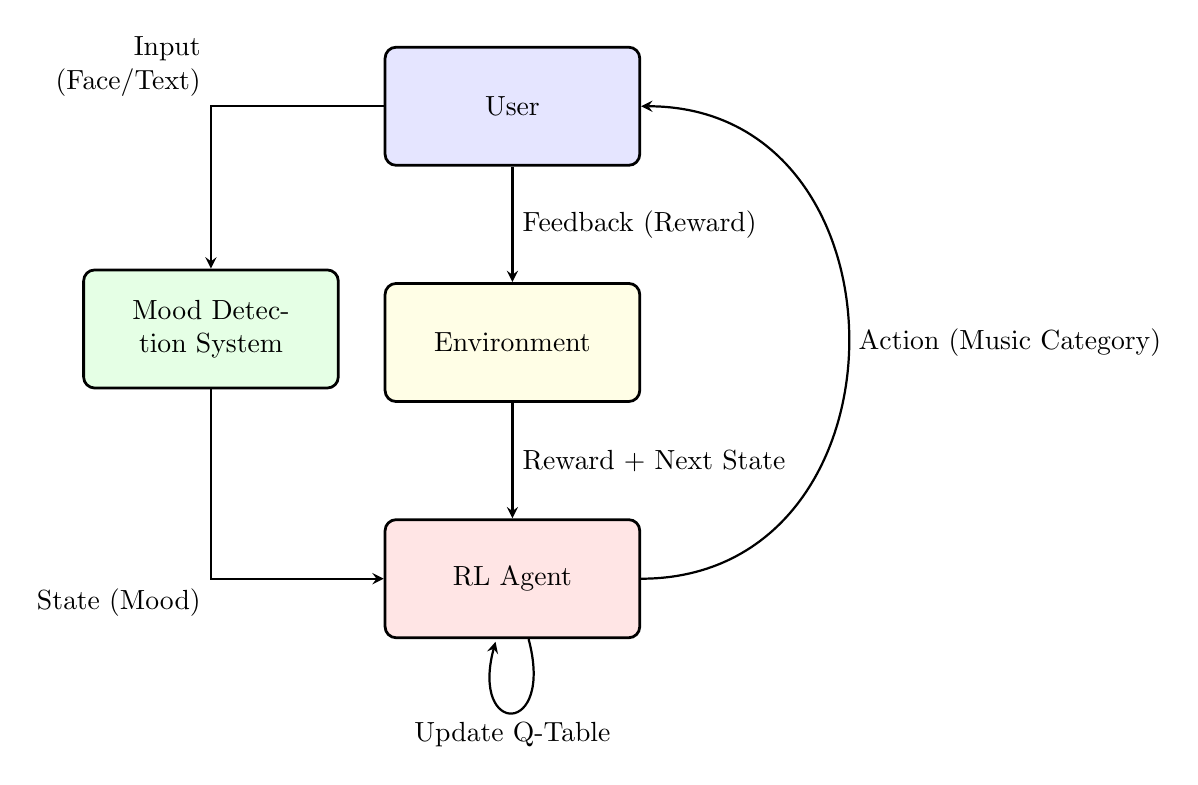
\begin{tikzpicture}[node distance=2.5cm, auto, >=stealth]
        % Styles
        \tikzstyle{block} = [rectangle, draw, fill=gray!10, text width=3cm, text centered, rounded corners, minimum height=1.5cm, line width=1pt]
        \tikzstyle{line} = [draw, thick, ->]

        % Nodes
        \node (user) [block, fill=blue!10] {User};
        \node (mood_sys) [block, fill=green!10, below left of=user, node distance=4cm, xshift=-1cm] {Mood Detection System};
        \node (env) [block, fill=yellow!10, below of=user, node distance=3cm] {Environment};
        \node (agent) [block, fill=red!10, below of=env, node distance=3cm] {RL Agent};

        % Edges matching the image
        % 1. User -> Mood Detection
        \path [line] (user) -| node [above left, text width=2cm, align=right] {Input (Face/Text)} (mood_sys);
        
        % 2. Mood Detection -> RL Agent
        \path [line] (mood_sys) |- node [below left] {State (Mood)} (agent);

        % 3. User -> Environment
        \path [line] (user) -- node [right] {Feedback (Reward)} (env);

        % 4. Environment -> RL Agent
        \path [line] (env) -- node [right] {Reward + Next State} (agent);

        % 5. RL Agent -> User (Action) - Curved arrow back to top
        \path [line] (agent.east) to [out=0, in=0, looseness=1.5] node [right] {Action (Music Category)} (user.east);

        % 6. RL Agent -> Self Loop (Update Q-Table)
        \path [line] (agent) edge [loop below] node {Update Q-Table} (agent);

    \end{tikzpicture}
    }
    \end{center}
    \small
    The architecture integrates Mood Detection and Reinforcement Learning in a continuous feedback loop.
\end{frame}

% Slide 4: User Walkthrough
\section{Workflow}
\begin{frame}{User Walkthrough}
    \begin{enumerate}
        \item \textbf{Step 1: Mood Input} \\
        User types "I feel energetic" or selects a mood (Happy, Sad, etc.).
        \item \textbf{Step 2: Recommendation} \\
        System predicts the best song genre/track for that mood.
        \item \textbf{Step 3: Playback \& Interaction} \\
        Song plays. User can \textbf{Like (+)}, \textbf{Dislike (-)}, or \textbf{Skip}.
        \item \textbf{Step 4: Adaptation} \\
        System updates its policy instantly based on the interaction.
    \end{enumerate}
\end{frame}

% Slide 5: Mood Detection Module
\section{Mood Detection}
\begin{frame}{Mood Detection Logic}
    We map user input to key musical features (Energy, Valence).
    
    \begin{table}
        \centering
        \begin{tabular}{l c c l}
            \toprule
            \textbf{Mood} & \textbf{Valence} & \textbf{Energy} & \textbf{Target Genre} \\
            \midrule
            Happy & High & High & Pop, Dance \\
            Sad & Low & Low & Acoustic, Ballad \\
            Energetic & High & Very High & Rock, EDM \\
            Calm & High & Low & Lo-Fi, Classical \\
            \bottomrule
        \end{tabular}
    \end{table}
\end{frame}

% Slide 6: Mood Transition Logic (NEW)
\section{Mood Transitions}
\begin{frame}{Mood Transition Dynamics}
    The system tracks how user interaction affects their \textbf{Next State} ($S_{t+1}$).
    
    \begin{block}{Transition Probability Matrix ($P$)}
        Example rules for state transitions based on Feedback ($F$):
    \end{block}

    \begin{table}
        \centering
        \small
        \begin{tabular}{l l l l}
            \toprule
            \textbf{Current State ($S_t$)} & \textbf{Action/Feedback ($F$)} & \textbf{Next State ($S_{t+1}$)} & \textbf{Logic / Probability} \\
            \midrule
            Happy & Dislike ("Wrong Vibe") & Angry & High Prob (Frustration) \\
            Sad & Skip (Fast) & Sad & Remains Sad (Searching) \\
            Sad & Like / Listen & Calm & Improved Mood \\
            Energetic & Like & Happy & Maintains Energy \\
            \bottomrule
        \end{tabular}
    \end{table}
    
    \textit{*This dynamic allows the agent to not just match the current mood, but steer the user towards a better one.*}
\end{frame}

% Slide 7: The RL Agent (Core)
\section{RL Agent}
\begin{frame}{Reinforcement Learning Model}
    The "Brain" of the system relies on Q-Learning.
    
    \begin{itemize}
        \item \textbf{Objective}: Maximize cumulative reward $R$ over time.
        \item \textbf{Q-Function}: $Q(s, a)$ estimates the value of picking song $a$ in mood $s$.
    \end{itemize}

    \begin{block}{Q-Learning Update Rule}
        \[
        Q(s, a) \leftarrow (1-\alpha)Q(s,a) + \alpha \left[ r + \gamma \max_{a'} Q(s', a') \right]
        \]
    \end{block}

    \begin{itemize}
        \item $\alpha$ (Learning Rate): 0.1 (Stable learning)
        \item $\gamma$ (Discount Factor): 0.9 (Long-term focus)
        \item $\epsilon$ (Exploration): Decays 1.0 $\to$ 0.1
    \end{itemize}
\end{frame}

% Slide 8: Reward System
\section{Reward System}
\begin{frame}{Reward System Design}
    Correctly defining rewards is critical for agent behavior.
    
    \begin{itemize}
        \item \textbf{Positive Feedback (+20)}: 
        User clicks "Add to Playlist" or "Love". Strong signal of success.
        \item \textbf{Passive Acceptance (+1)}: 
        User finishes the song without skipping.
        \item \textbf{Negative Feedback (-10)}:
        User clicks "Dislike", "Wrong Vibe", or "Skip".
    \end{itemize}

    \begin{figure}[h]
        \centering
        % Placeholder for Q-Table Heatmap
        \fbox{\begin{minipage}[c][3cm]{0.8\textwidth}
            \centering \vfill \textbf{<INSERT Q-TABLE HEATMAP IMAGE HERE>} \\
            \small Shows learned Q-values for (Mood vs. Genre) \vfill
        \end{minipage}}
        \caption{Visualization of Learned Agent Preferences (Q-Table)}
    \end{figure}
\end{frame}

% Slide 9: Simulation
\section{Simulation}
\begin{frame}{Simulation & Pre-training}
    To avoid the "Cold Start" problem, we train offline.
    
    \begin{itemize}
        \item \textbf{Simulated User}: A programmatic user with defined preferences.
        \item \textbf{Cycles}: 200+ Episodes in $<5$ seconds.
    \end{itemize}
    
    \begin{figure}[h]
        \centering
        % Placeholder for Mood Distribution
        \fbox{\begin{minipage}[c][3cm]{0.5\textwidth}
            \centering \vfill \textbf{<INSERT MOOD DIST. IMAGE>} \vfill
        \end{minipage}}
        \caption{Mood Distribution during Training}
    \end{figure}
\end{frame}

% Slide 10: Performance Results
\section{Performance}
\begin{frame}{Performance Analysis: Learning Curve}
    \begin{center}
    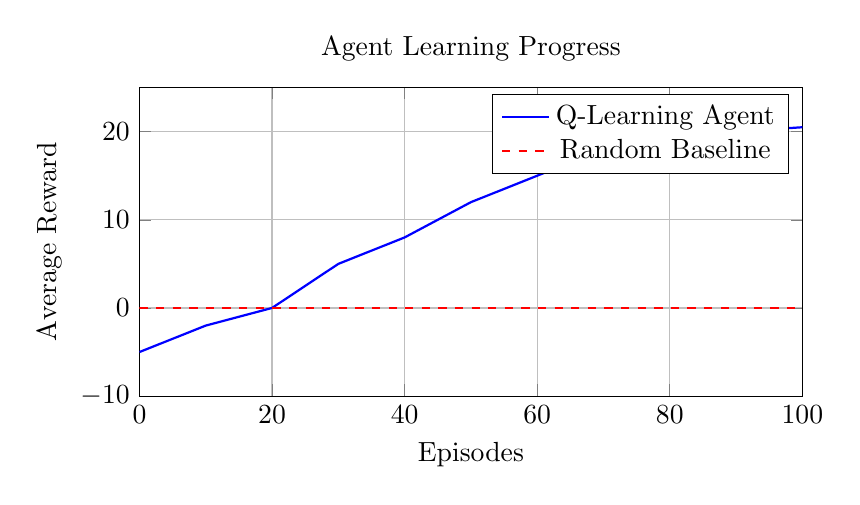
\begin{tikzpicture}
        \begin{axis}[
            width=10cm, height=5.5cm,
            xlabel={Episodes},
            ylabel={Average Reward},
            grid=major,
            ymin=-10, ymax=25,
            xmin=0, xmax=100,
            title={Agent Learning Progress}
        ]
        % Approximated learning curve
        \addplot[color=blue, mark=none, thick] coordinates {
            (0,-5) (10, -2) (20, 0) (30, 5) (40, 8) (50, 12) (60, 15) (70, 18) (80, 19) (90, 20) (100, 20.5)
        };
        \addlegendentry{Q-Learning Agent}
        
        \addplot[color=red, dashed, thick] coordinates { (0,0) (100,0) };
        \addlegendentry{Random Baseline}
        \end{axis}
    \end{tikzpicture}
    \end{center}
    The clear upward trend demonstrates effective learning of user preferences.
\end{frame}

% Slide 11: UI Implementation
\section{UI Implementation}
\begin{frame}{User Interface (Streamlit)}
    \begin{columns}
        \column{0.6\textwidth}
        \begin{itemize}
            \item \textbf{Real-Time Dashboard}:
            \begin{itemize}
                \item Current Track & Album Art.
                \item "Brain Power" Graph (Live Agent Status).
            \end{itemize}
            \item \textbf{Controls}:
            \begin{itemize}
                \item Like / Dislike Feedback Buttons.
                \item Playlist Manager.
            \end{itemize}
        \end{itemize}
        \column{0.4\textwidth}
        \centering
        % Placeholder for UI Screenshot
        \fbox{\begin{minipage}[c][4cm]{0.9\textwidth}
            \centering \vfill \textbf{<INSERT UI SCREENSHOT>} \vfill
        \end{minipage}}
    \end{columns}
\end{frame}

% Slide 12: Conclusion
\section{Conclusion}
\begin{frame}{Conclusion & Future Scope}
    \textbf{Summary}
    \begin{itemize}
        \item Successfully implemented RL-based personalized music recommendation.
        \item Agent learns from sparse feedback signals (Likes/Skips).
    \end{itemize}
    
    \vspace{0.3cm}
    \textbf{Future Work}
    \begin{itemize}
        \item \textbf{Deep RL}: DQN for high-dimensional state spaces.
        \item \textbf{Context Awareness}: Using time of day / location.
    \end{itemize}
    
    \vspace{0.5cm}
    \centering
    \Large \textbf{Thank You!} \\
    \small Questions?
\end{frame}

\end{document}
